\documentclass[a4paper,DIV=12,english]{scrartcl}
\usepackage[utf8]{inputenc}
\usepackage{graphicx}
\usepackage{hyperref}
\usepackage{csquotes}
\usepackage{amsthm}
\usepackage{amssymb}
\usepackage{bbm}
\usepackage{amsmath}
\usepackage{tikz}
\usepackage{svg}
\usepackage{braket}
\usepackage{caption}
\usepackage{subcaption}
\usepackage{placeins}
\usepackage[backend=bibtex]{biblatex}
% Fakesection
\newcommand{\fakesection}[1]{%
    \par\refstepcounter{section}                                        % Increase section counter
    \sectionmark{#1}                                                    % Add section mark (header)
    \addcontentsline{toc}{section}{\protect\numberline{\thesection}#1}  % Add section to ToC
    % Add more content here, if needed.
} 

\renewcommand{\thesubsection}{\thesection.\alph{subsection}}

\title{Data and Signal Analysis\\Problem Sheet 4}
\author{Elise Pilgermann, Max Maschke}
\date{\today}

\begin{document}
\maketitle

\section{The Message}
The ciphertext message gained from the signal reads \enquote{Caesar says: LZLVKBRXDPHUUBFKULVWPDVDQGDKDSSBQHZBHDU}. The plaintext can be recovered by a Caesar cipher shift by three characters, reading \enquote{IWISHYOUAMERRYCHRISTMASANDAHAPPYNEWYEAR}.

\section{Method}
\begin{figure}[h]
    \centering
    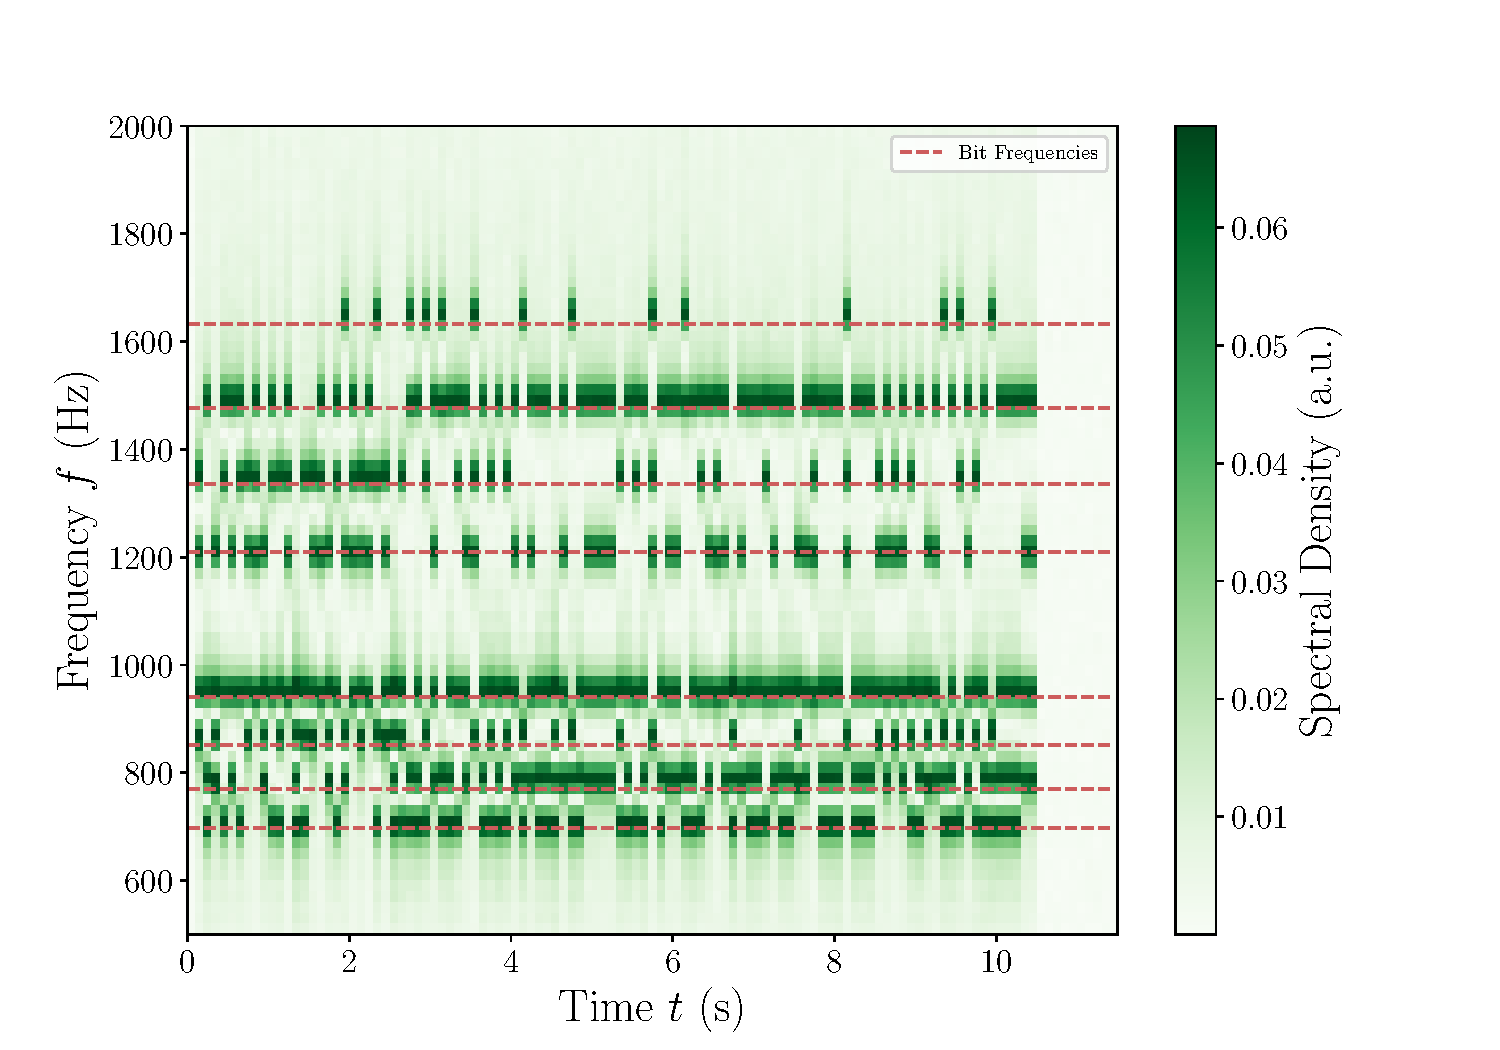
\includegraphics[width=0.7\textwidth]{../test.pdf}
    \caption{Short-time spectral density of the truncated signal.}
    \label{fig:stft}
\end{figure}
First, we truncate the first second of the signal because it does not contain any information. Then, we get the short time FT, using a 400 step, i.e. 50 ms, hamming window and a hop of 50 ms. This ensures that one FT is taken per symbol. We use \texttt{fft\_mode="onesided2X"} and \texttt{scale\_to="psd"} in \texttt{scipy}'s \texttt{ShortTimeFFT} class to get the spectral density. The results are shown in figure~\ref{fig:stft} and one can clearly see the structure of the signal. To decode it, we get a binary mask by extracting all elements where the spectral density is greater than 0.35, see figure~\ref{fig:mask}.
\begin{figure}
    \centering
    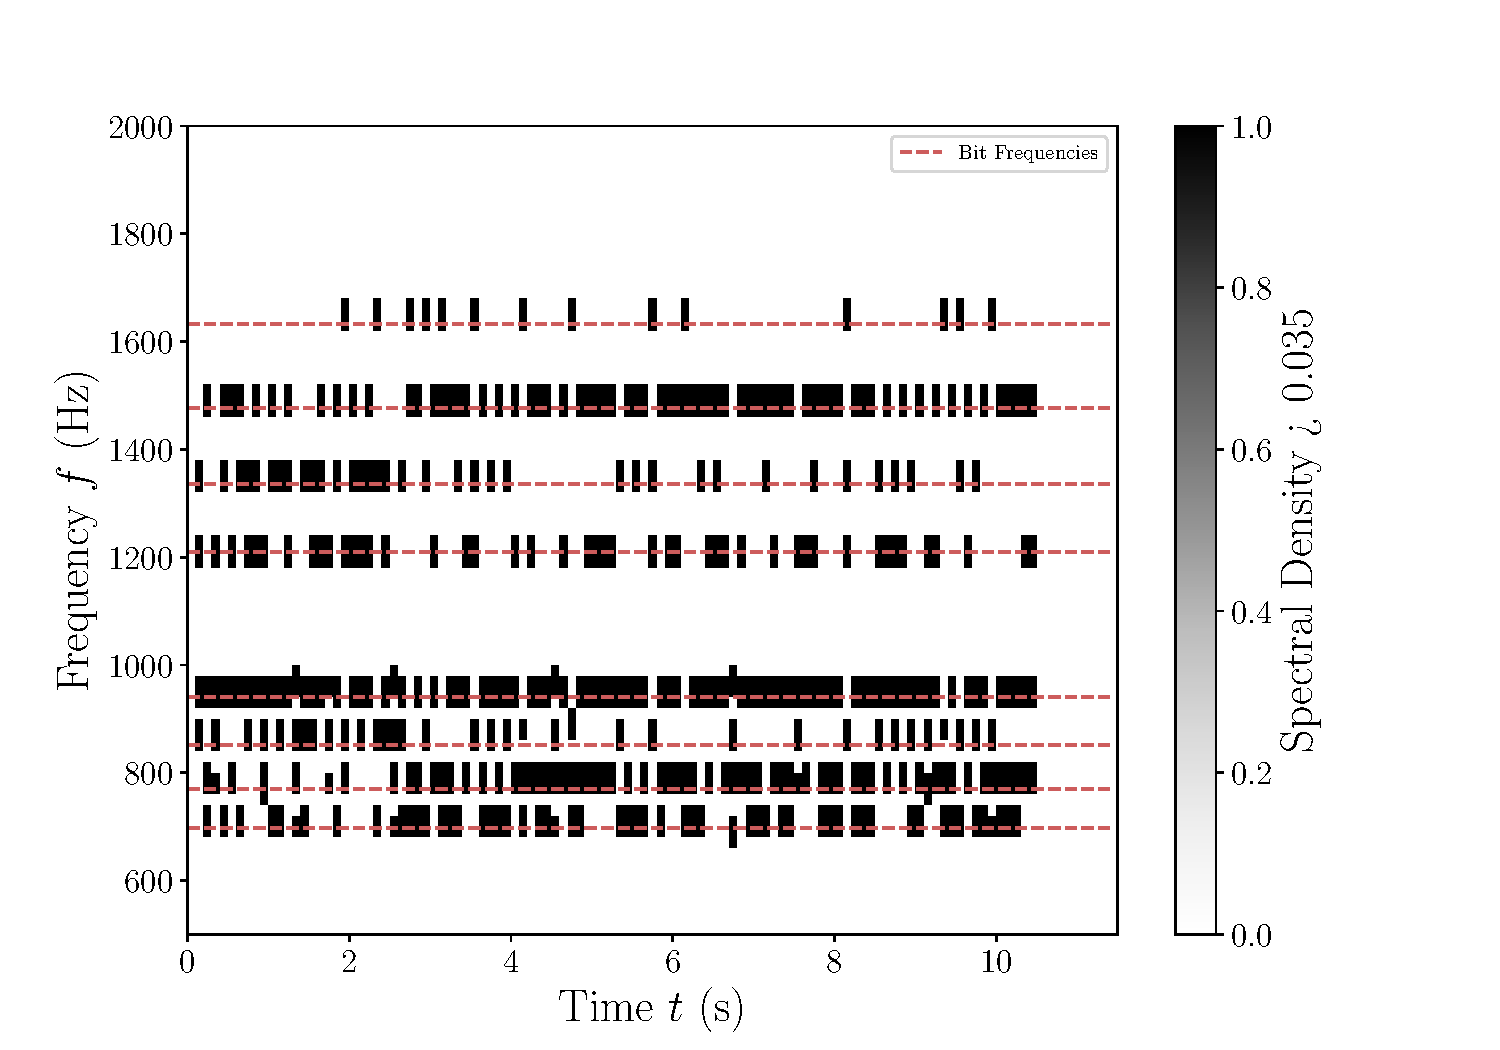
\includegraphics[width=0.7\textwidth]{../test2.pdf}
    \caption{Binary mask of the spectral density compared to the arbitrary threshold 0.35.}
    \label{fig:mask}
\end{figure}
We can then iterate through the columns of the mask at the indices corresponding to the signal frequencies, setting the bits of a zero-initialised integer according to the rules given in the exercise. Combining all characters into a string yields the ciphertext message.


\end{document}